\begin{appendices}

% =========================================================
% APPENDIX A
% =========================================================

\chapter{Project Planning}

% ---------------------------------------------------------
\section{Project Timeline}

The EvoRAG project development was initiated during Semester VI following the project timeline illustrated in Figure A.1. 
The completed work in this phase includes problem identification, literature survey, requirement analysis, system architecture design, and initial implementation of the retrieval and multi-persona reasoning modules. 
Further development, testing, optimization, dashboard integration, and final deployment will be continued in the upcoming semester.

\vspace{0.5cm}

\begin{figure}[H]
    \centering
    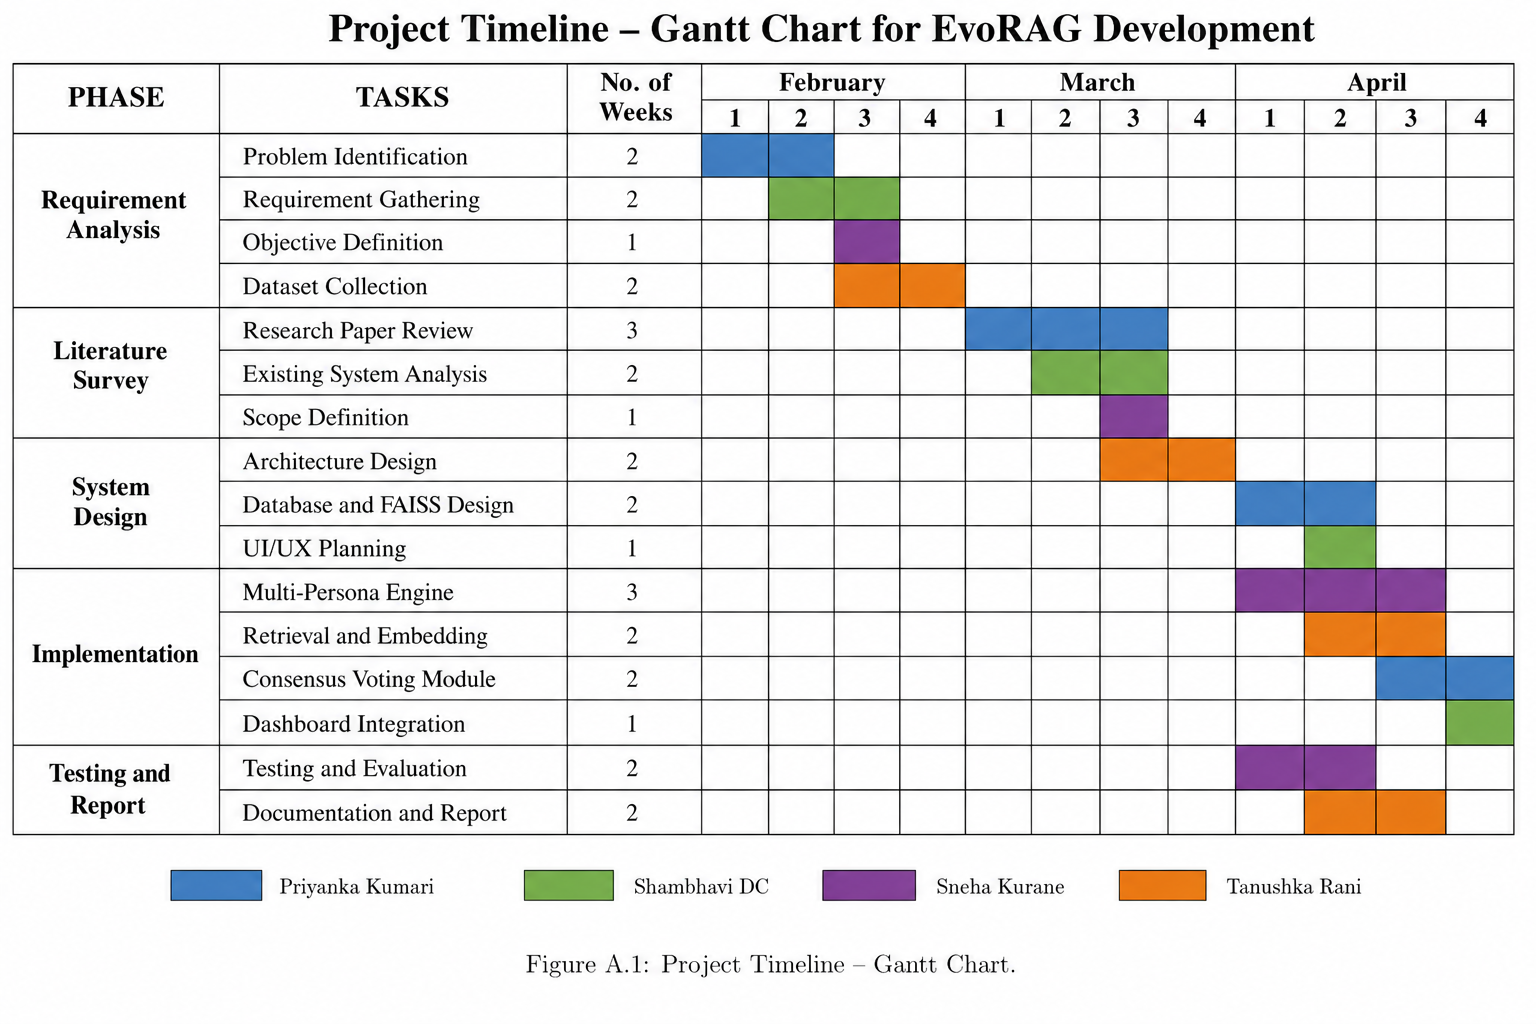
\includegraphics[width=\linewidth]{timeline.png}
    \caption{Project Timeline -- Gantt Chart}
    \label{fig:timeline}
\end{figure}

\clearpage

% ---------------------------------------------------------
\section{Budget Estimation}

This section presents the estimated budget required for the development and deployment of the EvoRAG system. 
The budget mainly includes software tools, API usage, cloud resources, development infrastructure, and miscellaneous expenses incurred during the project implementation.

\vspace{0.5cm}

\begin{table}[H]
\centering
\renewcommand{\arraystretch}{1.3}

\begin{tabular}{|c|p{8cm}|c|}
\hline

\textbf{SL. NO.} &
\centering \textbf{Software / Resources} &
\textbf{Estimated Cost [INR]}
\tabularnewline

\hline

1 & Development System and Internet Resources & 15,000 \\
\hline

2 & NewsAPI Subscription / API Usage & 2,000 \\
\hline

3 & GNews API and RSS Feed Integration & 1,500 \\
\hline

4 & Python Libraries and Development Tools & 0 (Open Source) \\
\hline

5 & FAISS Vector Database Setup & 0 (Open Source) \\
\hline

6 & Sentence Transformer Models & 0 (Open Source) \\
\hline

7 & Local LLM Deployment and Testing & 3,000 \\
\hline

8 & Frontend Dashboard Development & 2,500 \\
\hline

9 & Testing, Evaluation and Documentation & 2,000 \\
\hline

10 & Miscellaneous Expenses & 1,500 \\
\hline

\multicolumn{2}{|c|}{\textbf{Total Estimated Cost}} &
\textbf{27,500 INR} \\
\hline

\end{tabular}

\vspace{0.5cm}

\caption{Budget Estimation for the EvoRAG Project}
\label{tab:budget_estimation}

\end{table}

% =========================================================
% APPENDIX B
% =========================================================

\chapter{Dataset and Input Details}

The EvoRAG system utilizes a dynamic knowledge ingestion pipeline to ensure that retrieved information remains current, reliable, and contextually relevant for every user query. 
The dataset is generated dynamically at runtime using multiple live data sources instead of relying on static pre-trained corpora.

The system gathers information from APIs such as NewsAPI and GNews API along with trusted RSS feeds. 
The collected data undergoes cleaning, deduplication, chunking, and embedding generation before being stored in a FAISS vector database for semantic retrieval.

The input pipeline supports:
\begin{itemize}
    \item Real-time query-based data collection
    \item Data cleaning using BeautifulSoup
    \item Sliding-window chunking strategy
    \item Embedding generation using sentence-transformers
    \item Efficient vector search using FAISS indexing
\end{itemize}

% =========================================================
% APPENDIX C
% =========================================================

\chapter{Configuration Details}

This appendix provides the technical configuration and environment details required to execute the EvoRAG system efficiently.

The project was developed using Python and integrated with various libraries and frameworks for vector retrieval, multi-persona reasoning, and dashboard visualization.

\textbf{Hardware Requirements}
\begin{itemize}
    \item Intel Core i7 / AMD Ryzen 7 Processor
    \item Minimum 16GB RAM
    \item SSD Storage
    \item NVIDIA GPU (recommended for faster inference)
\end{itemize}

\textbf{Software Requirements}
\begin{itemize}
    \item Python 3.10+
    \item FAISS Vector Database
    \item LangChain Framework
    \item Ollama for Local LLM Execution
    \item BeautifulSoup4 and Pandas
    \item SQLite Database
\end{itemize}

\textbf{Environment Setup}
\begin{enumerate}
    \item Clone the repository: \texttt{git clone https://github.com/prowessclust/evorag}
    \item Create a virtual environment: \texttt{python -m venv venv}
    \item Activate the environment and install dependencies: \texttt{pip install -r requirements.txt}
    \item Configure the local LLM via Ollama: \texttt{ollama pull mistral} or \texttt{ollama pull llama3}
\end{enumerate}

\textbf{Project Repository}

The complete project source code and implementation details are maintained in the GitHub repository.

\begin{center}
\url{https://github.com/prowessclust/evorag}
\end{center}

\end{appendices}